% !TEX encoding = UTF-8
% !TEX TS-program = pdflatex
% !TEX root = ../tesi.tex
% !TEX spellcheck = it-IT

%**************************************************************
\chapter{Verifica e validazione}
\label{cap:verifica-validazione}
%**************************************************************

\section{Test di unità}
L'approccio Test Driven garantisce intrinsecamente che ogni unità software sia testata ancora prima della sua implementazione. Ogni unità dovrebbe contenere il quantitativo minimo di codice necessario a far rendere positivo il test ideato e scritto in precedenza.\\
Questo approccio, sebbene all'inizio sia piuttosto insolito ed a prima vista tedioso, risulta invece essere imprescindibile nello sviluppo di applicazioni web, soprattutto utilizzando framework JavaScript. AngularJS stesso è stato pensato per scrivere applicazioni facilmente testabili, includendo al suo interno delle librerie create appositamente per il testing.\\
Mi è stato quindi possibile testare ogni componente della logica dell'applicazione, controllando il comportamento delle unità e dei loro metodi. Tramite l'utilizzo di sistemi di automazione, nel mio caso \emph{Karma}, sono riuscito a rendere il processo di testing quanto più automatico possibile ed a calcolare con facilità le metriche base per verificare l'utilità dei test scritti.\\
Tramite il plugin di \emph{coverage} di Karma, ho generato automaticamente tali cifre, suddividendole per:
\begin{itemize}
	\item line coverage;
	\item statement coverage;
	\item branch coverage;
	\item function coverage.
\end{itemize}
Nella figura sottostante, presento i dati in forma tabellare, come vengono visualizzati dall'output del plugin \emph{karma-coverage}, installabile facilmente da \gls{npm}.

%DA CAMBIARE LA WIDTH, PERCHE' COSI' FA' CAGARE, PLZ. >_<
\begin{figure}[!h] 
    \centering 
    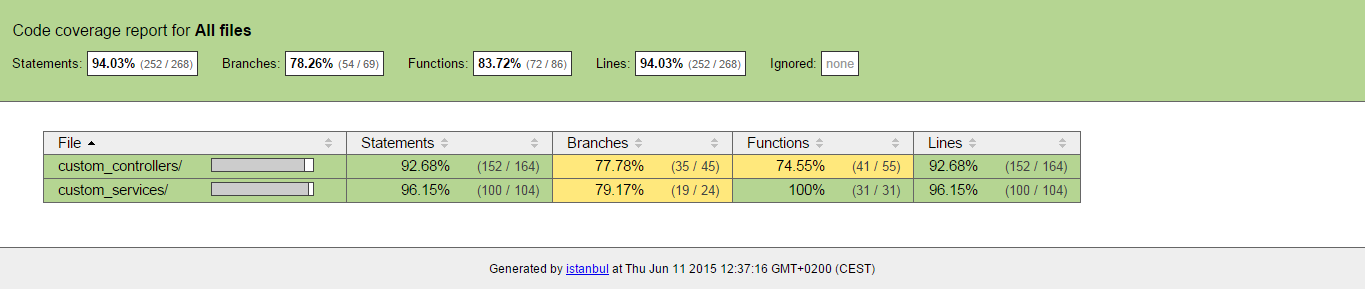
\includegraphics[width=0.9\columnwidth]{coverage/coverage_all} 
    \caption{Metriche di copertura generali nel progetto SkillMatrix}
\end{figure}

\begin{figure}[!h] 
    \centering 
    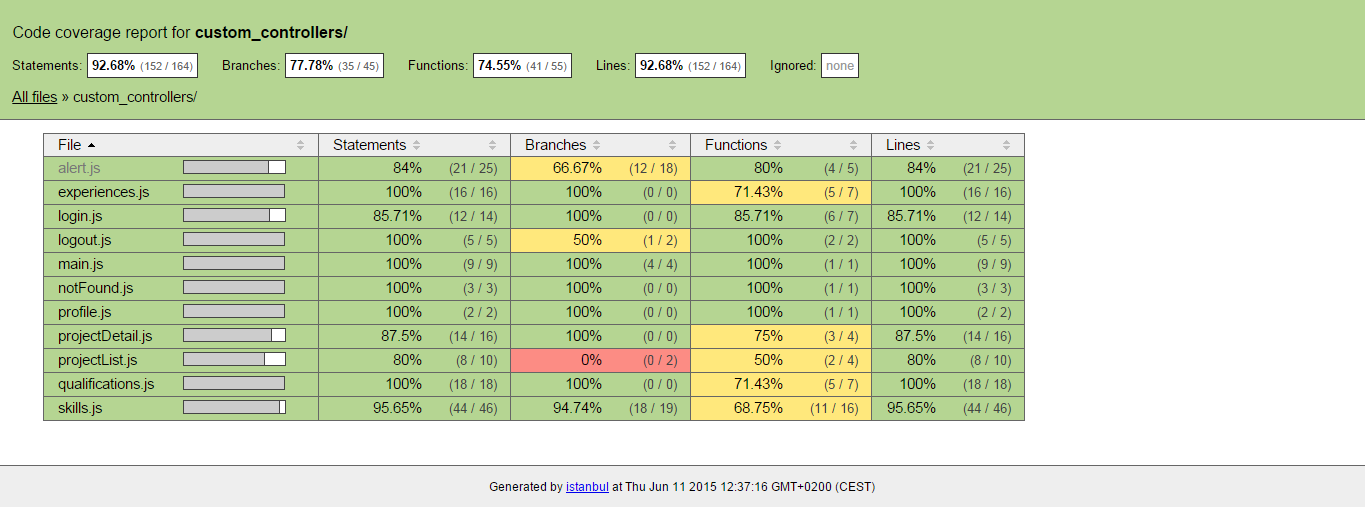
\includegraphics[width=0.9\columnwidth]{coverage/coverage_controllers} 
    \caption{Metriche di copertura dei controller nel progetto SkillMatrix}
\end{figure}

\begin{figure}[!h] 
    \centering 
    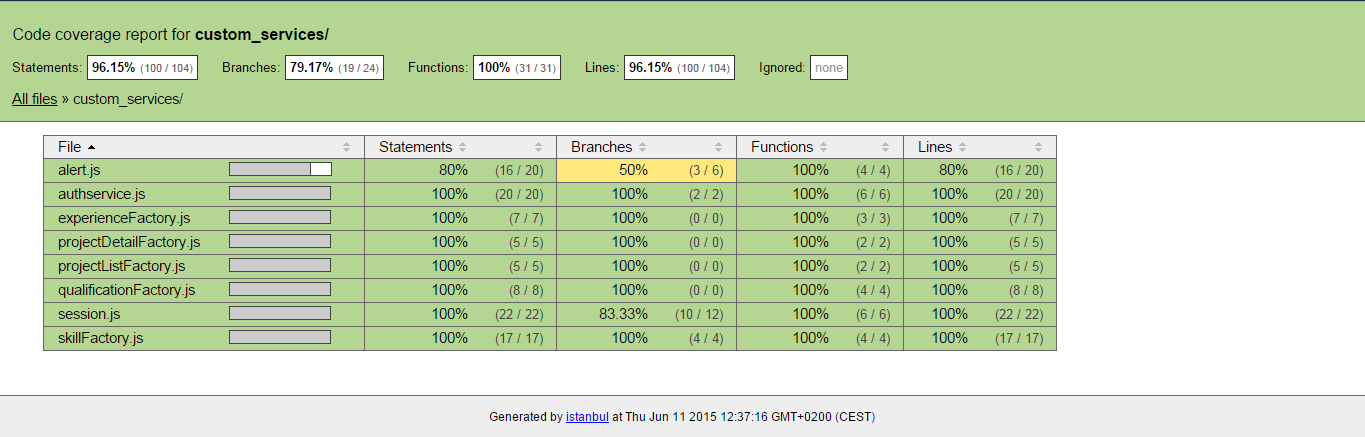
\includegraphics[width=0.9\columnwidth]{coverage/coverage_services} 
    \caption{Metriche di copertura dei servizi nel progetto SkillMatrix}
\end{figure}

%**************************************************************

\newpage

\section{Test End-To-End}
I test di scenario (o \gls{e2e}) servono a verificare la corretta interazione di uno o più unità software al fine di perseguire una certa azione dell'utente. AngularJS consiglia di utilizzare lo stack fornito da \emph{Protractor} e da \emph{Selenium} per automatizzare il processo di testing. Ogni test di scenario automatizza gli input utente in un browser ed analizza gli output ad ogni modifica.\\
Questi test sono molto più laboriosi di un test di unità eseguito con \emph{Karma}, ma sono molto più vicini ad essere dei test di validazione.\\
In questo progetto ho creato un test per ogni tipo di azione utente, dalla semplice consultazione di informazioni del profilo all'inserimento di una nuova \emph{skill} nel sistema. Ogni test avviene automatizzando l'input attraverso la selezione dei vari elementi \gls{html} della pagina a cui fa riferimento il test e gli elementi vengono individuati tramite semplici selettori \gls{css} o \emph{jQuery}.\\

\begin{figure}[!h] 
    \centering 
    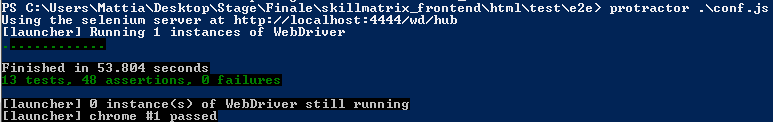
\includegraphics[width=0.9\columnwidth]{e2e} 
    \caption{Grafica da console dell'esecuzione di test e2e di Protractor}
\end{figure}

Ogni test è composto di passi ben precisi, ovvero le stesse azioni che compongono l'input utente. Il test quindi deve effettuare gli stessi passi, compresi i singoli click su dei link e l'input di testo quando richiesto. La prossima porzione di codice è il test \gls{e2e} del login, sia errato che corretto, con le proprie \emph{expectations}, ovvero i valori previsti in output.

\begin{verbatim}
'use strict';

describe('SkillMatrix login', function() {

  beforeEach(function() {
    browser.get('base.html');
    browser.waitForAngular();
  });

  it('should have a title', function() {
    expect(browser.getTitle()).toEqual('SkillMatrix');
  });

  it('should appear an error message on wrong login', function() {
    element(by.model('credentials.name')).sendKeys('IKS');
    element(by.model('credentials.password')).sendKeys(2);

    element(by.css('button[type="submit"]')).click();

    expect(element(by.binding('alert.message')).getText()).
        toEqual('I dati di autenticazione sono errati(1)');
  });

  it('should login correctly with right credentials', function() {
    element(by.model('credentials.name')).sendKeys('IKS');
    element(by.model('credentials.password')).sendKeys('pippo');

    element(by.css('button[type="submit"]')).click();

    browser.getLocationAbsUrl().then(function(url) {
        expect(url.split('#')[1]).toBe('/profile');
      });
  });
  
});
\end{verbatim}